\section{Auswertung}


\subsection{Untersuchung der Charakteristik des Zählrohres}
Die aufgenommen Messwerte für die Zählrate $N$ unter variabler Betriebspspannung $U$ sind
in Tabelle \ref{tab: zaelrate_strom} aufgeführt. Der angegebene Fehler wurde hierbei stets
auf eine ganze Zahl gerundet. Eine Darstellung der Messwerte befindet sich in Abbildung \ref{fig: zählrate_ges}.
Als obere und untere Schranke für die Betrachtung des Plateaus wurden die Werte zwischen $U = \SI{370}{\volt}$
und $U = \SI{600}{\volt}$ gewählt, da an den Grenzen dieses Intervalls ein signifikanter Unterschied zu einem
linearen Verlauf zu erkennen ist (vgl. die beiden benachbarten Werte in Abbildung \ref{}). Mittels linearer %\ref
Regressionsrechnung ergeben sich für die Steigung $m$ und den Ordinatenabschnitt $b$ folgende Werte
\begin{align}
  m &= \SI{0.041 \pm 0.009}{(\second\volt)^-1} \\
  b &= \SI{412 \pm 4}{\per\second}
\end{align}%.
Eine graphische Darstellung der Messwerte im gewählten Plateaubereich, sowie die Regressiongerade sind in
Abbildung \ref{fig: plateau} einzusehen.

\subsection{Bestimmung der Totzeit}
Mit Hilfe des Oszilloskops wurde die Totzeit fünf mal unter verschiedenen Betriebsspannungen ausgemessen. Die Messwerte
sind in Tabelle \ref{tab: totzeit_oszi} aufgetragen. Für den Mittelwert mit zugehöriger Standardabweichung ergibt sich
\begin{equation}
  T_1 = \SI{96 \pm 2}{\micro\second}.
\end{equation}
Für die Anwendung der Zwei-Quellen-Methode wurden jeweils mit der Betriebsspannung $U = \SI{480}{\volt}$ die
Impulszahlen $Z\ua{i}$ der Strahlung zweier einzelner Proben ($N_1,\, N_2$) und der Gesamtimpulszahl $Z\ua{1+2}$ aufgenommen.
\begin{align}
  Z_1 &= \SI{2.57(2)e+04}{}\\
  Z_2 &= \SI{1.11(3)e+03}{}\\
  Z_{1+2} &= \SI{2.68(2)e+04}{}
\end{align}%., da kann man auch num verwenden?
Mit dem Messintervall $\Delta t = \SI{60}{\second}$ ergeben sich somit für die Zählraten
\begin{align}
  N_1 &= \SI{428 \pm 3}{\per\second}\\
  N_2 &= \SI{19(0) }{\per\second}\\
  N_{1+2} &= \SI{446 \pm 3}{\per\second}
\end{align}%.
Auch hier wurde wieder auf eine ganze Zahl gerundet. Im Rahmen der Fehlertoleranz wird die Unleichung %Ungleichung
\eqref{} als erfüllt angenommen. Einsetzen der ungerundeten Werte in Gleichung \eqref{eq:totzeit} liefert damit die Totzeit %eqref{}
\begin{equation}
  T_2 = \SI{0.3(24)e+02}{\micro\second}.
\end{equation}
\begin{table} 
\centering 
\caption{Mit dem Oszilloskop gemessene Totzeiten $T$ unter verschiedenen Beschleunigungsspannungen $U$.} 
\label{tab: totzeit_oszi} 
\begin{tabular}{S S } 
\toprule  
{$U/ \si{\volt}$} & {$T/ \si{\micro\second}$}  \\ 
\midrule  
 360  & 100\\ 
400  & 90\\ 
460  & 90\\ 
500  & 100\\ 
540  & 100\\ 
\bottomrule 
\end{tabular} 
\end{table}
\begin{table} 
\centering 
\caption{Mit dem Oszilloskop gemessene Erholungszeiten $T_E$ unter verschiedenen Beschleunigungsspannungen $U$.} 
\label{tab: erholungszeit} 
\begin{tabular}{S S } 
\toprule  
{$U/ \si{\volt}$} & {$T_E/ \si{\micro\second}$}  \\ 
\midrule  
 520  & 300\\ 
540  & 250\\ 
570  & 250\\ 
630  & 300\\ 
640  & 300\\ 
\bottomrule 
\end{tabular} 
\end{table}

\subsection{Bestimmung der Erholungszeit}
Für die Erholungszeit $T\ua{E}$ wurden die in Tabelle \ref{} dokumentierten Werte mit dem Oszilloskop ausgemessen. Als %\ref{}
Mittelwert mit Standardabweichung berechnet sich
\begin{equation}
  T_E = \SI{2.8(1)e+02}{\micro\second}.
\end{equation}

\subsection{Bestimmung der pro Teilchen vom Zählrohr freigesetzten Ladungsmenge}
Die gemessenen mittleren Ströme $I$, sowie die gemäß \eqref{} berechneten Ladungsmengen $\Delta Q$, die pro %\eqref{}
Teilchen im Zählrohr freigesetzt werden, sind in Tabelle \ref{tab: zaelrate_strom} eingetragen. In Abbildung
\ref{fig: ladung} befindet sich eine Auftragung der Ladungsmenge gegen die Beschleunigungsspannung $U$.


\newpage
\input{table/zählrate_strom_ladung.tex}
\begin{figure}
  \centering
  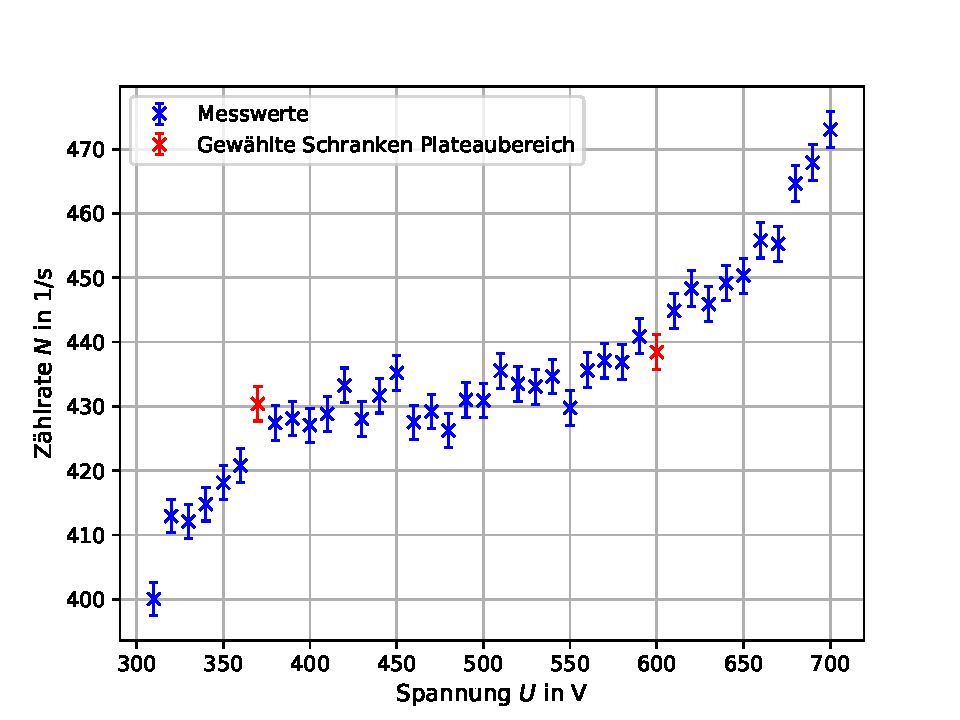
\includegraphics[width = 0.8\textwidth]{../Messdaten/plots/all_counts.pdf}
  \caption{Graphische Darstellung der Zählrohrcharakteristik, Abhängigkeit der Zählrate $N$ von der Betriebsspannung $U$.}
  \label{fig: zählrate_ges}
\end{figure}
\begin{figure}
  \centering
  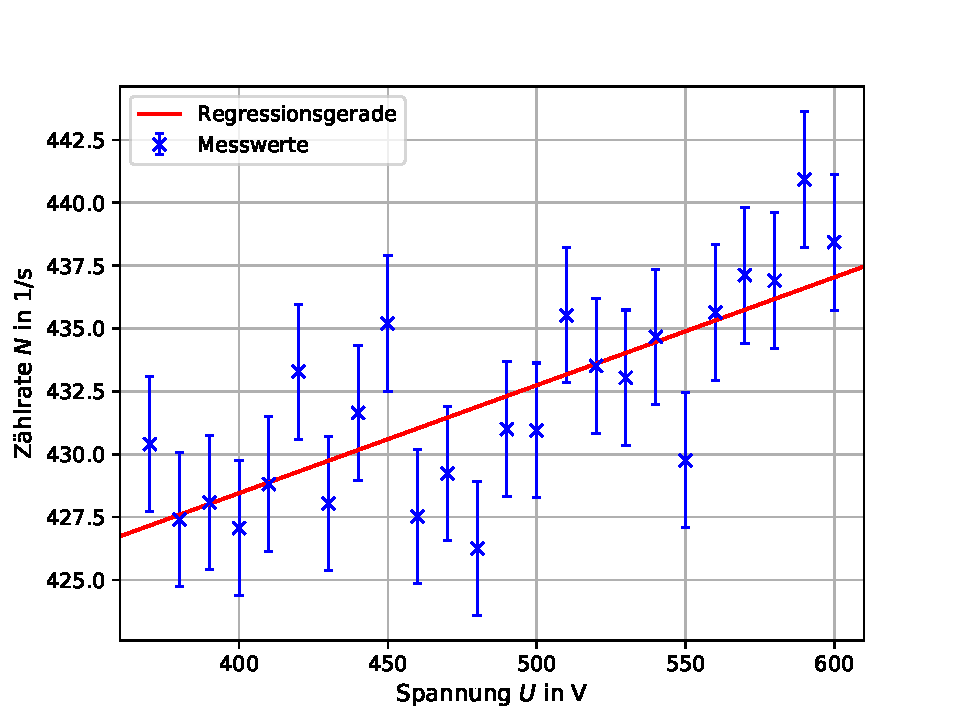
\includegraphics[width = 0.8\textwidth]{../Messdaten/plots/plateau.pdf}
  \caption{Graphische Darstellung des Plateaubereichs.}
  \label{fig: plateau}
\end{figure}
\begin{figure}
  \centering
  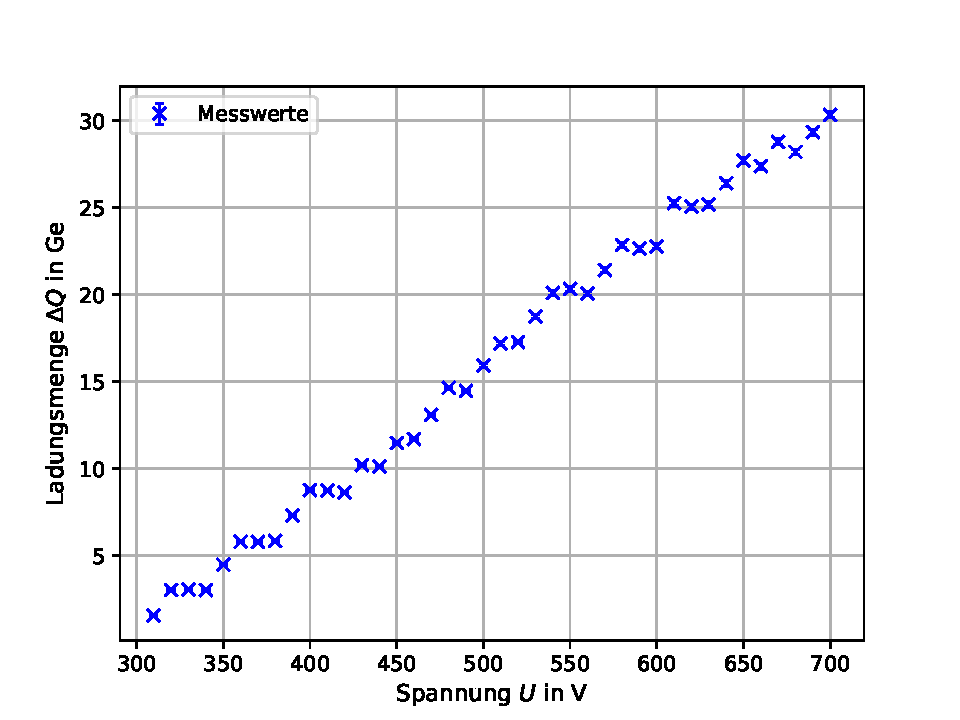
\includegraphics[width = 0.8\textwidth]{../Messdaten/plots/ladung.pdf}
  \caption{Graphische Darstellung der Abhängigkeit zwischen Zählrohrspannung $U$ und pro einfallendem Teilchen ausgelöster Ladungsmenge $\Delta Q$.}
  \label{fig: ladung}
\end{figure}
